\chapter{hugoについて}
hugoは静的なWebジェネレーターということで、軽く環境構築をしていきましょう。

\section{勉強資料}
  \url{https://youtu.be/hjD9jTi_DQ4}

\section{環境構築}
とりあえず、hugoをインストールしてみましょう。

  \begin{shaded}
    \begin{verbatim}
    $ brew install hugo
    \end{verbatim}
  \end{shaded}
  たったこれだけで完成です。

\section{hugoプロジェクト作成}
  あらかじめ、レポジトリを作成しておきましょう。
  githubからクローンをして、レポジトリを持ってきてください。

  \begin{shaded}
    \begin{verbatim}
    git clone 自分のリポジトリのURL

    cd クローンしたディレクトリ
    \end{verbatim}
  \end{shaded}

    では、次にhugoのプロジェクトを作成します。

  \begin{shaded}
    \begin{verbatim}
    ❯ hugo new site hugo-demo -f yml
    Congratulations! Your new Hugo site is created in /Users/k22120kk/Downloads/hugo-demo.

    Just a few more steps and you're ready to go:

    1. Download a theme into the same-named folder.
      Choose a theme from https://themes.gohugo.io/ or
      create your own with the "hugo new theme <THEMENAME>" command.
    2. Perhaps you want to add some content. You can add single files
      with "hugo new <SECTIONNAME>/<FILENAME>.<FORMAT>".
    3. Start the built-in live server via "hugo server".

    Visit https://gohugo.io/ for quickstart guide and full documentation.
    \end{verbatim}
  \end{shaded}

  \begin{figure}[H]
    \centering
    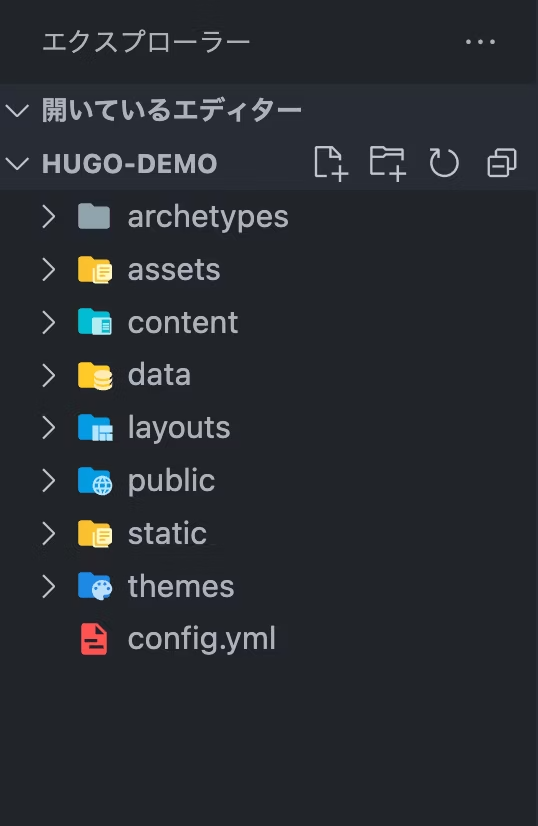
\includegraphics[width=8cm]{./image/02-chap5/filetree.png}
    \caption{実際に用いた技術構成の図}
    \label{chap5-firetree-image}
  \end{figure}

\section{テーマの設定}
  \subsection{テーマの選択}
    hugoではテーマを用いることで簡単にそれっぽいWebページを作成することができます。
    \url{https://themes.gohugo.io/}
    この中から気に入ったテーマを探してみてください。
    注意:テーマによって若干設定項目が変わる場所があるので気をつけてください。
    では今回は下記のテーマを用いて作成していこうと思います。
    \url{https://themes.gohugo.io/themes/hugo-theme-stack/}

    ちなみに、各テーマに大体ドキュメントがありますので、そのstartedなどをみることをお勧めします。
    今回のドキュメントはこちらになります。
    \url{https://stack.jimmycai.com/}

  \subsection{テーマの反映}
    では、ドキュメントの指示に従いながら、テーマの反映を行っていきます。
    \url{https://stack.jimmycai.com/guide/getting-started}

    cdを用いて、hugoのプロジェクトページまできてください。
    下記を実行することでテーマを反映させることができます。

    \begin{shaded}
      \begin{verbatim}
        git submodule add https://github.com/CaiJimmy/hugo-theme-stack/ themes/hugo-theme-stack
      \end{verbatim}  
    \end{shaded}

    git initをしていない場合はこちらで実行してみてください。

    \begin{shaded}
      \begin{verbatim}
        git clone https://github.com/CaiJimmy/hugo-theme-stack/ themes/hugo-theme-stack
      \end{verbatim}  
    \end{shaded}
    
    そうすることにより、themesディレクトリが作成されて、テーマの素材が入ります。

    \begin{figure}[H]
      \centering
      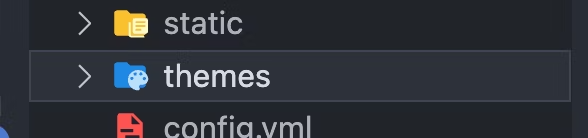
\includegraphics[width=8cm]{./image/02-chap5/firetree-themes.png}
      \caption{themesフォルダーができている様子の図}
      \label{chap5-firetree-themes-image}
    \end{figure}

    では、configファイルを設定して、themeを設定しましょう

    \begin{tcolorbox}[breakable]
      \begin{verbatim}
        baseURL: ""
        languageCode: ja
        title: My New Hugo Site
        theme: hugo-theme-stack
      \end{verbatim}
    \end{tcolorbox}

    では、実際に動かしてみて、動作するか確認してみましょう。

    \begin{shaded}
      \begin{verbatim}
        ❯ hugo server
        Start building sites … 
        hugo v0.108.0+extended darwin/arm64 BuildDate=unknown
        WARN 2022/12/23 10:44:43 found no layout file for "HTML" for kind "taxonomy": You should create a template file which matches Hugo Layouts Lookup Rules for this combination.
        WARN 2022/12/23 10:44:43 found no layout file for "HTML" for kind "home": You should create a template file which matches Hugo Layouts Lookup Rules for this combination.
        WARN 2022/12/23 10:44:43 found no layout file for "HTML" for kind "taxonomy": You should create a template file which matches Hugo Layouts Lookup Rules for this combination.

                          | EN  
        -------------------+-----
          Pages            |  3  
          Paginator pages  |  0  
          Non-page files   |  0  
          Static files     |  0  
          Processed images |  0  
          Aliases          |  0  
          Sitemaps         |  1  
          Cleaned          |  0  

        Built in 6 ms
        Watching for changes in /Users/k22120kk/Downloads/hugo-demo/{archetypes,assets,content,data,layouts,static}
        Watching for config changes in /Users/k22120kk/Downloads/hugo-demo/config.yml
        Environment: "development"
        Serving pages from memory
        Running in Fast Render Mode. For full rebuilds on change: hugo server --disableFastRender
        Web Server is available at http://localhost:1313/ (bind address 127.0.0.1)
        Press Ctrl+C to stop
      \end{verbatim}  
    \end{shaded}

    ウェブブラウザでhttp://localhost:1313/ をURLに入れて読み込んでみましょう。

    下のような画像が出力されれば成功です。

    \begin{figure}[H]
      \centering
      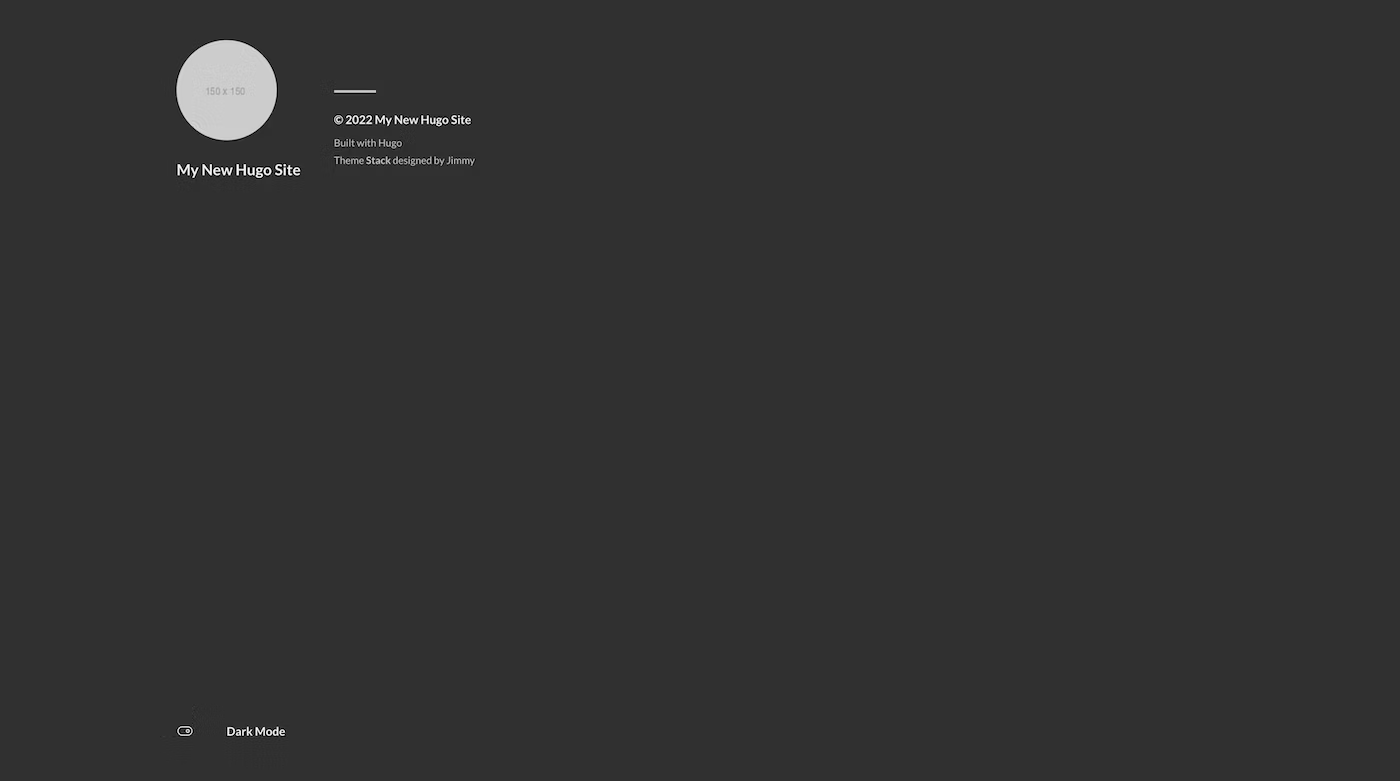
\includegraphics[width=8cm]{./image/02-chap5/output-homepage.png}
      \caption{テーマが反映された様子の図}
      \label{chap5-homepage-image}
    \end{figure}

  \subsection{Webページを作成してみる}
    では、軽くマークダウンを作成をしてWebページを作成してみましょう
    下のコマンドを入力して、マークダウンを作成してみましょう。

    \begin{shaded}
      \begin{verbatim}
        hugo new post/first.md
      \end{verbatim}
    \end{shaded}

    そうすると下記のようなファイルができているはずです。
    
    \begin{tcolorbox}[breakable]
      \begin{verbatim}
        ---
        title: "First"
        date: 2022-12-23T10:49:46+09:00
        draft: true
        ---
      \end{verbatim}
    \end{tcolorbox}

    それでは追加で書き加えてみます。
    ここで状態が編集モードになっているため、draft:trueをdraft:falseに変更しましょう。
    こうしないと、デプロイした時に表示されなくなります。

    \begin{tcolorbox}[breakable]
      \begin{verbatim}
        ---
        title: "First"
        date: 2022-12-23T10:49:46+09:00
        draft: false
        ---

        # 最初の書き込みです
        ここから僕だけのウェブサイトが生まれます。
      \end{verbatim}
    \end{tcolorbox}

    下のように、作成したWebページが作られているはずです。

    \begin{figure}[H]
      \centering
      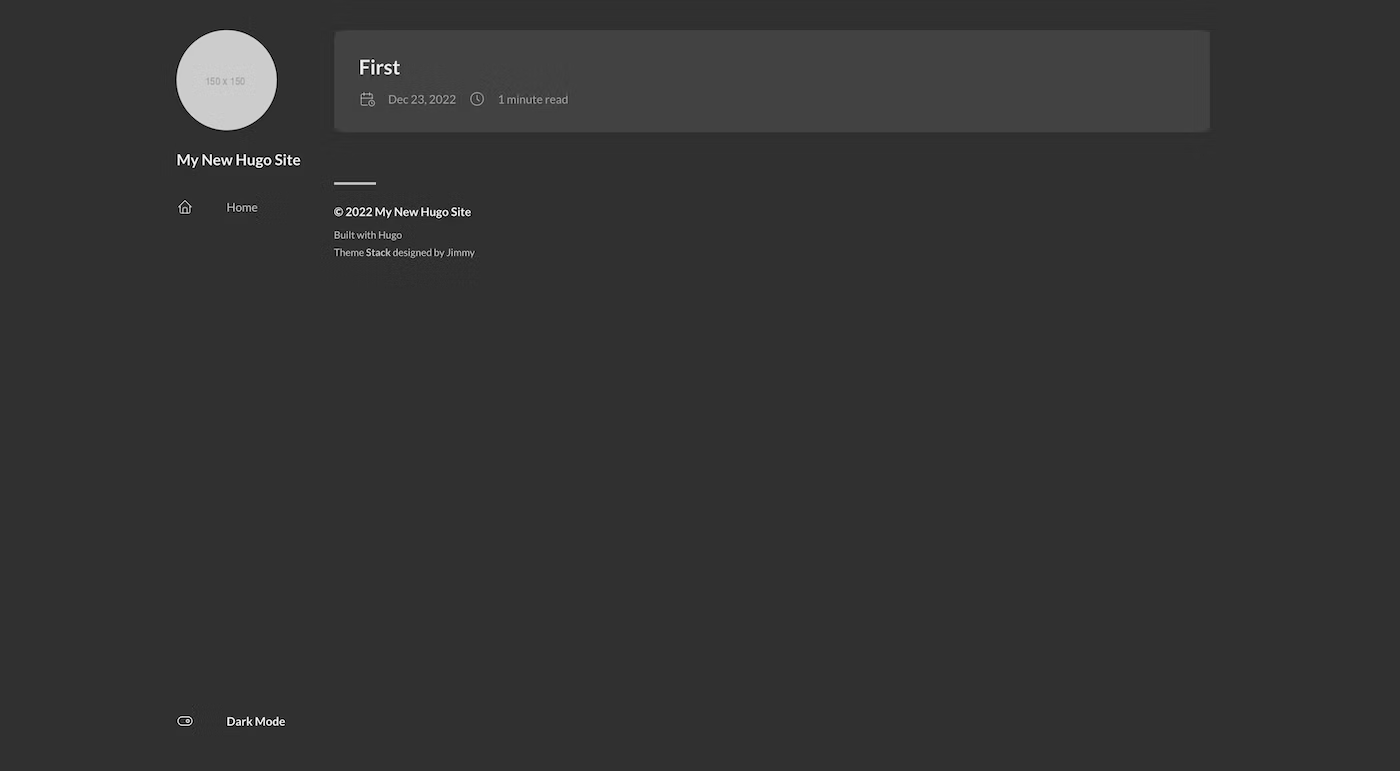
\includegraphics[width=8cm]{./image/02-chap5/add-file-list.png}
      \caption{ファイルが追加されている様子の図}
      \label{chap5-add-file-list-image}
    \end{figure}

    \begin{figure}[H]
      \centering
      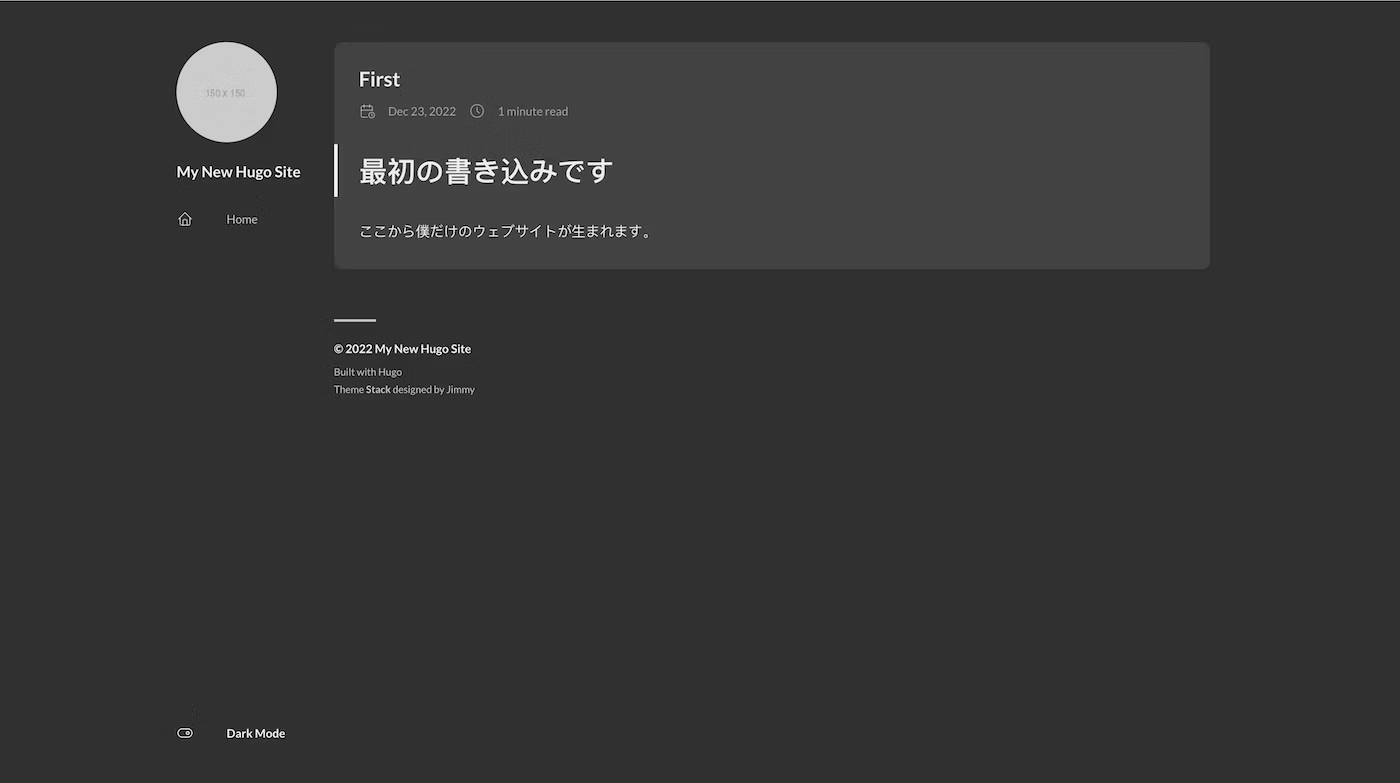
\includegraphics[width=8cm]{./image/02-chap5/add-file-content.png}
      \caption{ファイルの中身が追加されている様子の図}
      \label{chap5-add-file-content-image}
    \end{figure}

  \subsection{細かい設定など}
    ここでは、細かく説明はしませんが、configファイルや、mdファイルの上の部分で様々な設定をすることができます。
    詳しい説明をしてくれているWebページを紹介しますので、ぜひご自身で色々触って自分だけのオリジナルサイトを作ってみてください。

    \subsubsection{configの設定}
      \url{https://github.com/CaiJimmy/hugo-theme-stack/blob/master/exampleSite/config.yaml}

      \url{https://miiitomi.github.io/p/hugo/}

    \subsubsection{フロントマターの設定}
      \url{https://takaken.tokyo/dev/hugo/post/write-post/}

    




    
  


